\section{The ESP Cache Hierarchy}
\label{sec:cache}

Figure \ref{fig:esp_tile} shows an example of a 4x4 tile ESP system with
elements of the memory hierarchy highlighted; the heterogeneous mix of tiles are
connected by a multi-plane network-on-chip (NoC).

ESP's coherence protocol is implemented by the L2 and last-level caches.  Each
\emph{Processor Tile} contains an open-source core, instantiated off-the-shelf
with its own L1 cache. The ESP L2 allows different cores to seamlessly
participate in ESP's coherence protocol, despite having potentially different
ISAs, endianness, and interfaces.  \emph{Accelerator Tiles}, which instantiate
a \emph{loosely-coupled accelerator}, can also optionally be equipped with
their own private L2 cache, which allows them to also participate in the
coherence protocol, just like processor cores.

The \emph{Memory Tile} contains the LLC and directory controller, which manage
coherence among all L2 caches in the system, and a channel to external DRAM.
The LLC can be partitioned across multiple memory tiles in the system with each
partition serving a discrete partition of the global address space and
providing its own channel to DRAM. The LLC can also handle DMA requests
directly from accelerators, saving off-chip memory accesses in many
circumstances.

\par Compared to the L1 and L2 caches, the LLC contains additional metadata for
all cache lines active in the system at any point, such as which cores own or
share the cache line. These metadata are necessary for the execution of the
extended MESI directory-based cache coherence protocol.  In addition to the
standard MESI states (Modified, Exclusive, Shared, Invalid), the ESP coherence
protocol introduces a Valid state, which corresponds to lines that are not
owned or shared by any private cache. Maintaining a Valid state saves an
off-chip memory access to subsequent requests for this line; it is also used to
represent lines that have been accessed by an accelerator through DMA to the
LLC. Valid lines are also the first choices for evictions.

The various caches and processing elements in ESP communicate through the NoC.
Three NoC planes are used for coherence requests, responses, and forwards,
while two planes are used for DMA requests and responses from/to accelerators.

%\begin{figure}[h]
%  \centering
%  \captionsetup{justification=centering, format=hang}
%  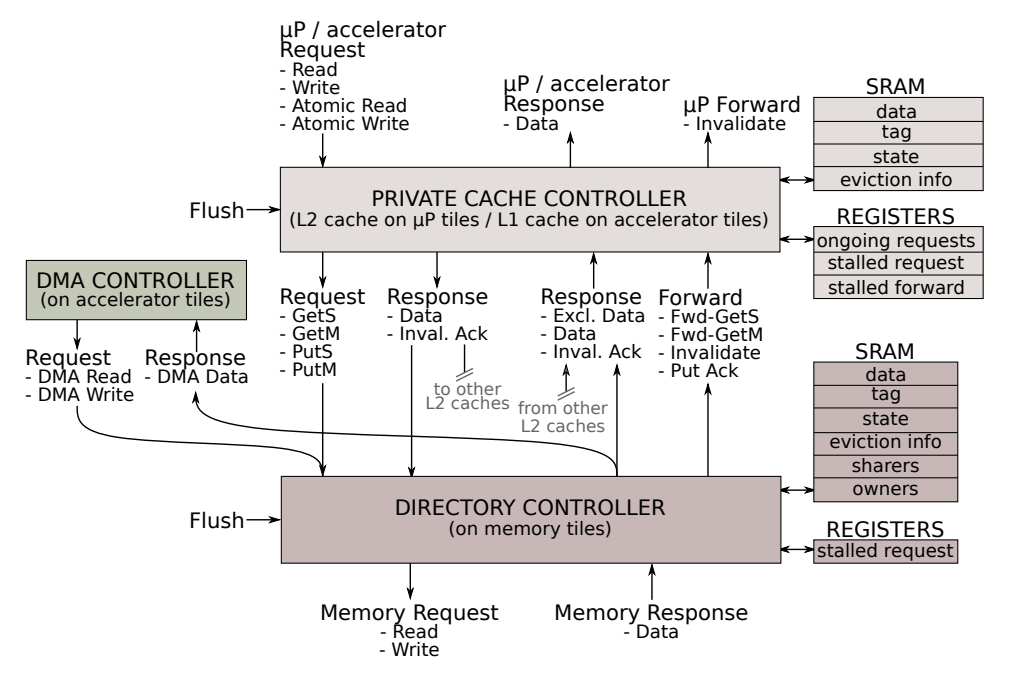
\includegraphics[width=1\columnwidth]{fig/esp_hier.png}
%  \caption{ESP Cache Hierarchy~\cite{giri18}}
%  \label{fig:esp_hier}
%  \end{figure}

\begin{figure}[t]
  \centering
  \captionsetup{justification=centering, format=hang}
  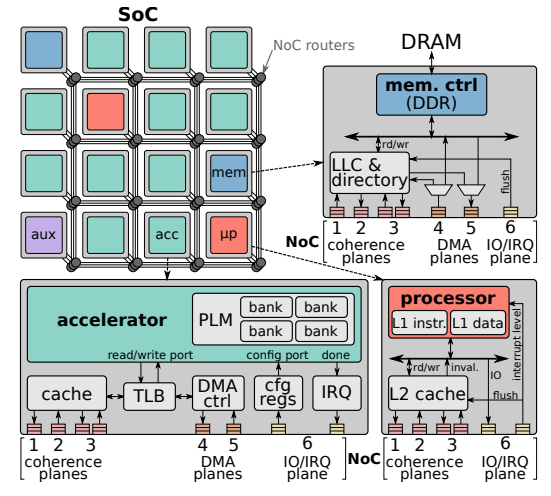
\includegraphics[width=1\columnwidth]{fig/noccache.png}
  \caption{Detailed ESP Tile Grid~\cite{giri18}}
  \label{fig:esp_tile}
  \end{figure}

